\section{RESCUER}
    \subsection{Home}
        \begin{figure}[H] \noindent \centering
            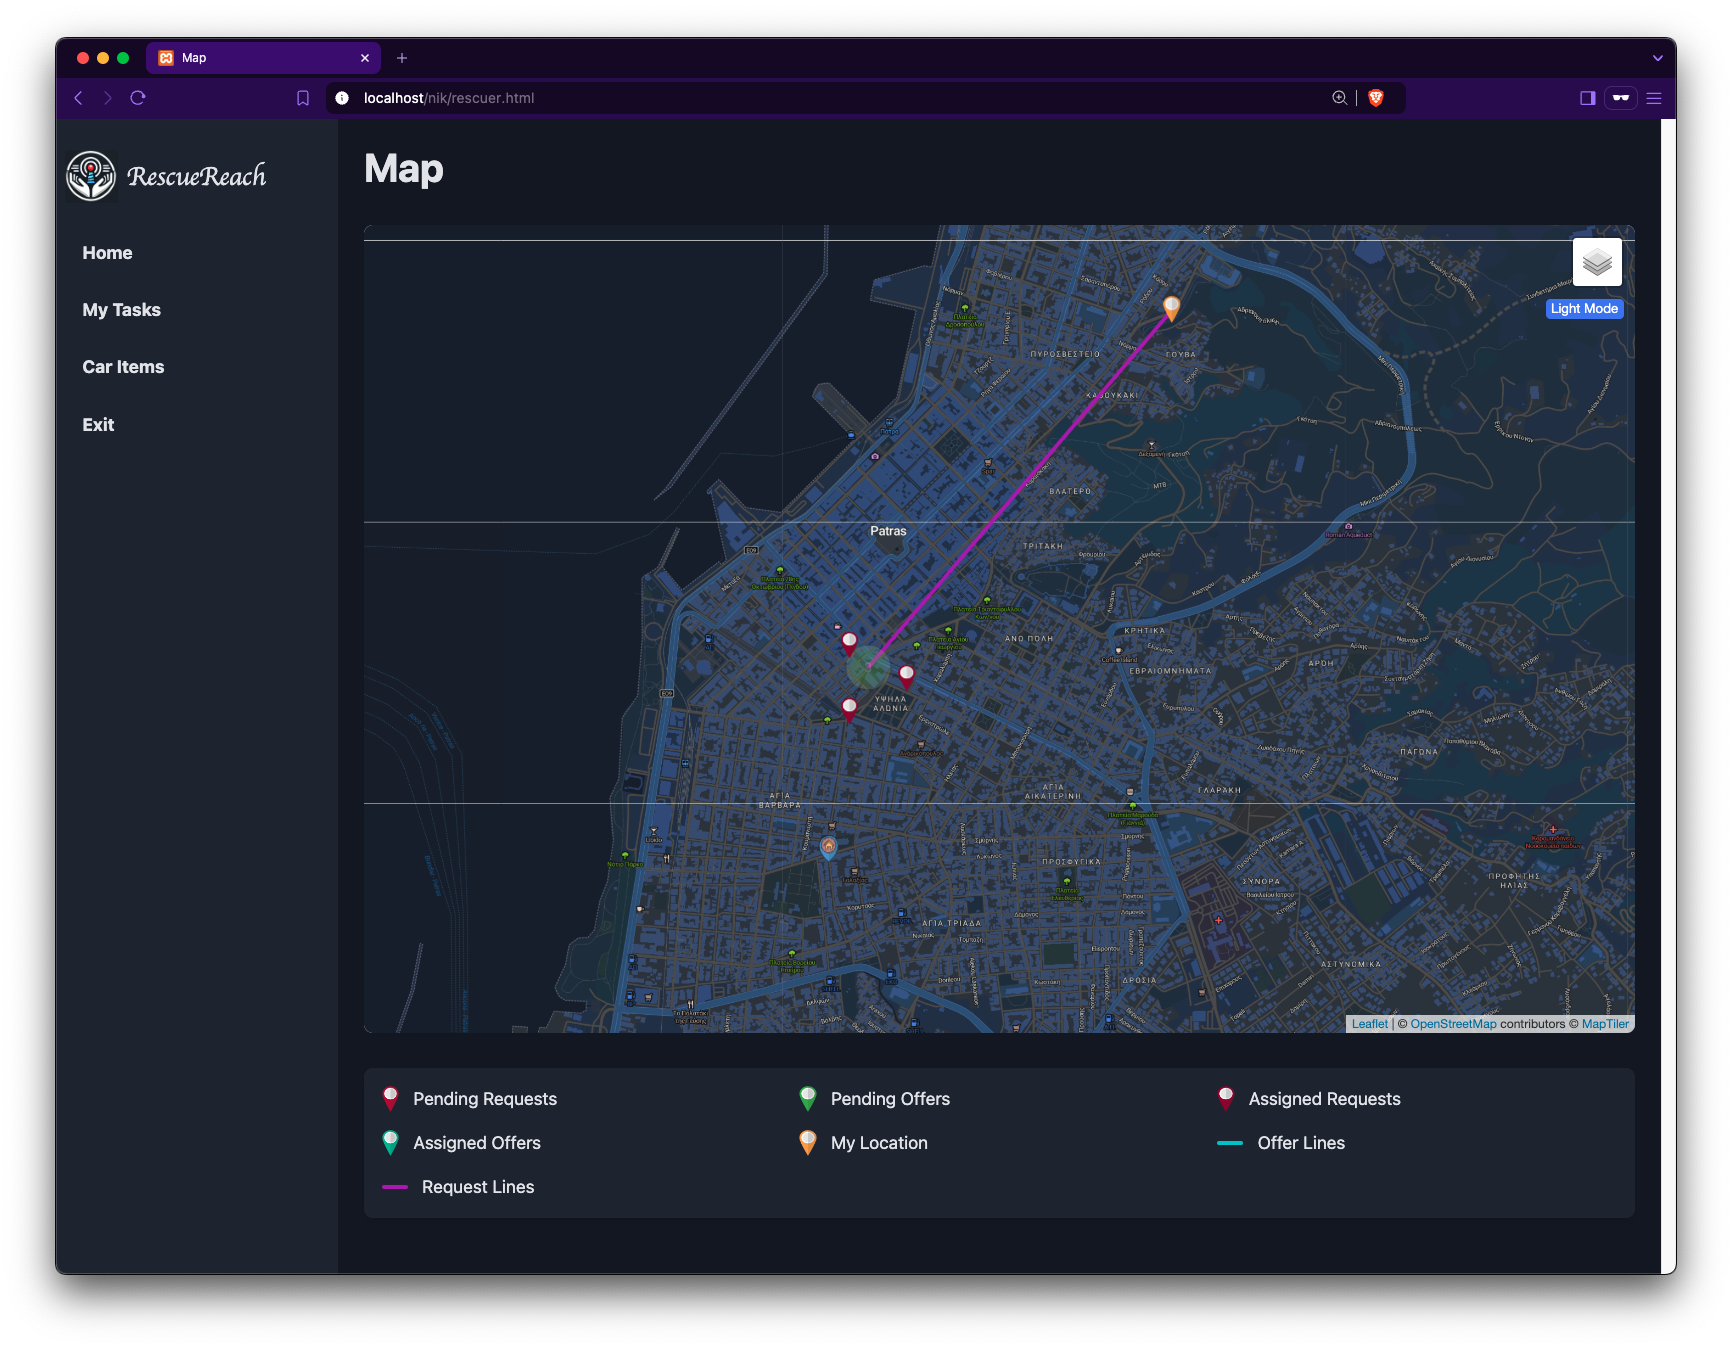
\includegraphics[width=0.8\textwidth]{img/rescuer-map}
            \caption{Αρχική σελίδα rescuer}
        \end{figure}

        Η αρχική σελίδα του διασώστη περιλαμβάνει το χάρτη της πόλης, με τα markers που αντιστοιχούν στα requests και τα offers των πολιτών.
        Ο rescuer δεν μπορεί να δει τους υπόλοιπους rescuers.
        Αυτό επιτυγχάνεται μέσω της \c{logged\_user} σταθεράς, που απομονώνει τον συγκεκριμένο χρήστη από τα δεδομένα που επιστρέφονται από τη βάση δεδομένων.
        Η διαδικασία εμφάνισης των markers είναι παρόμοια όπως στη σελίδα του admin.

        \begin{figure}[H] \noindent \centering
            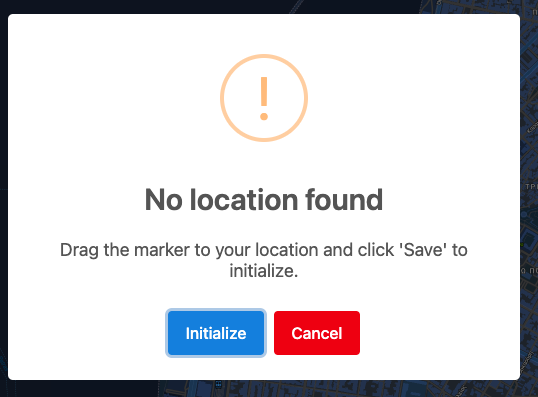
\includegraphics[width=0.4\textwidth]{img/rescuer-no_location}
            \caption{Αρχικοποίηση rescuer}
        \end{figure}

        Μια διαφορά που προκύπτει στην \c{fetchRescuerLocation()} είναι κατά την αρχικοποίηση της τοποθεσίας του διασώστη μετά την εγγραφή του από τον admin.

        \begin{figure}[H] \noindent \centering
            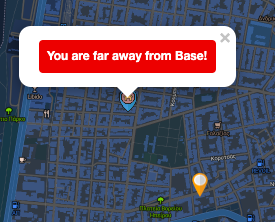
\includegraphics[width=0.3\textwidth]{img/rescuer-marker1}
            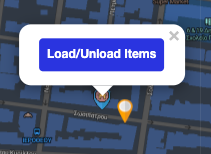
\includegraphics[width=0.3\textwidth]{img/rescuer-marker2}
            \caption{Ο διασώστης πρέπει να είναι σε ακτίνα 50m από τη βάση}
        \end{figure}

        Η \c{baseProximity()} ελέγχει την απόσταση του διασώστη από τη βάση και ανάλογα τροποποιεί το συννεφάκι της βάσης.
        Η \c{displayLines()} χρησιμοποιεί τις συντεταγμένες του διασώστη και των πολιτών και δημιουργεί γραμμές (\c{L.polyline}) μεταξύ τους.
        Τέλος, η \c{takeTask()} ελέγχει με AJAX request στην \c{takeTask.php} πόσα tasks έχουν ήδη επιλεγεί από τους διασώστες, και αν είναι πάνω από 4, δεν επιτρέπει την επιλογή ενός νέου.

    \subsection{My Tasks}
        \begin{figure}[H] \noindent \centering
            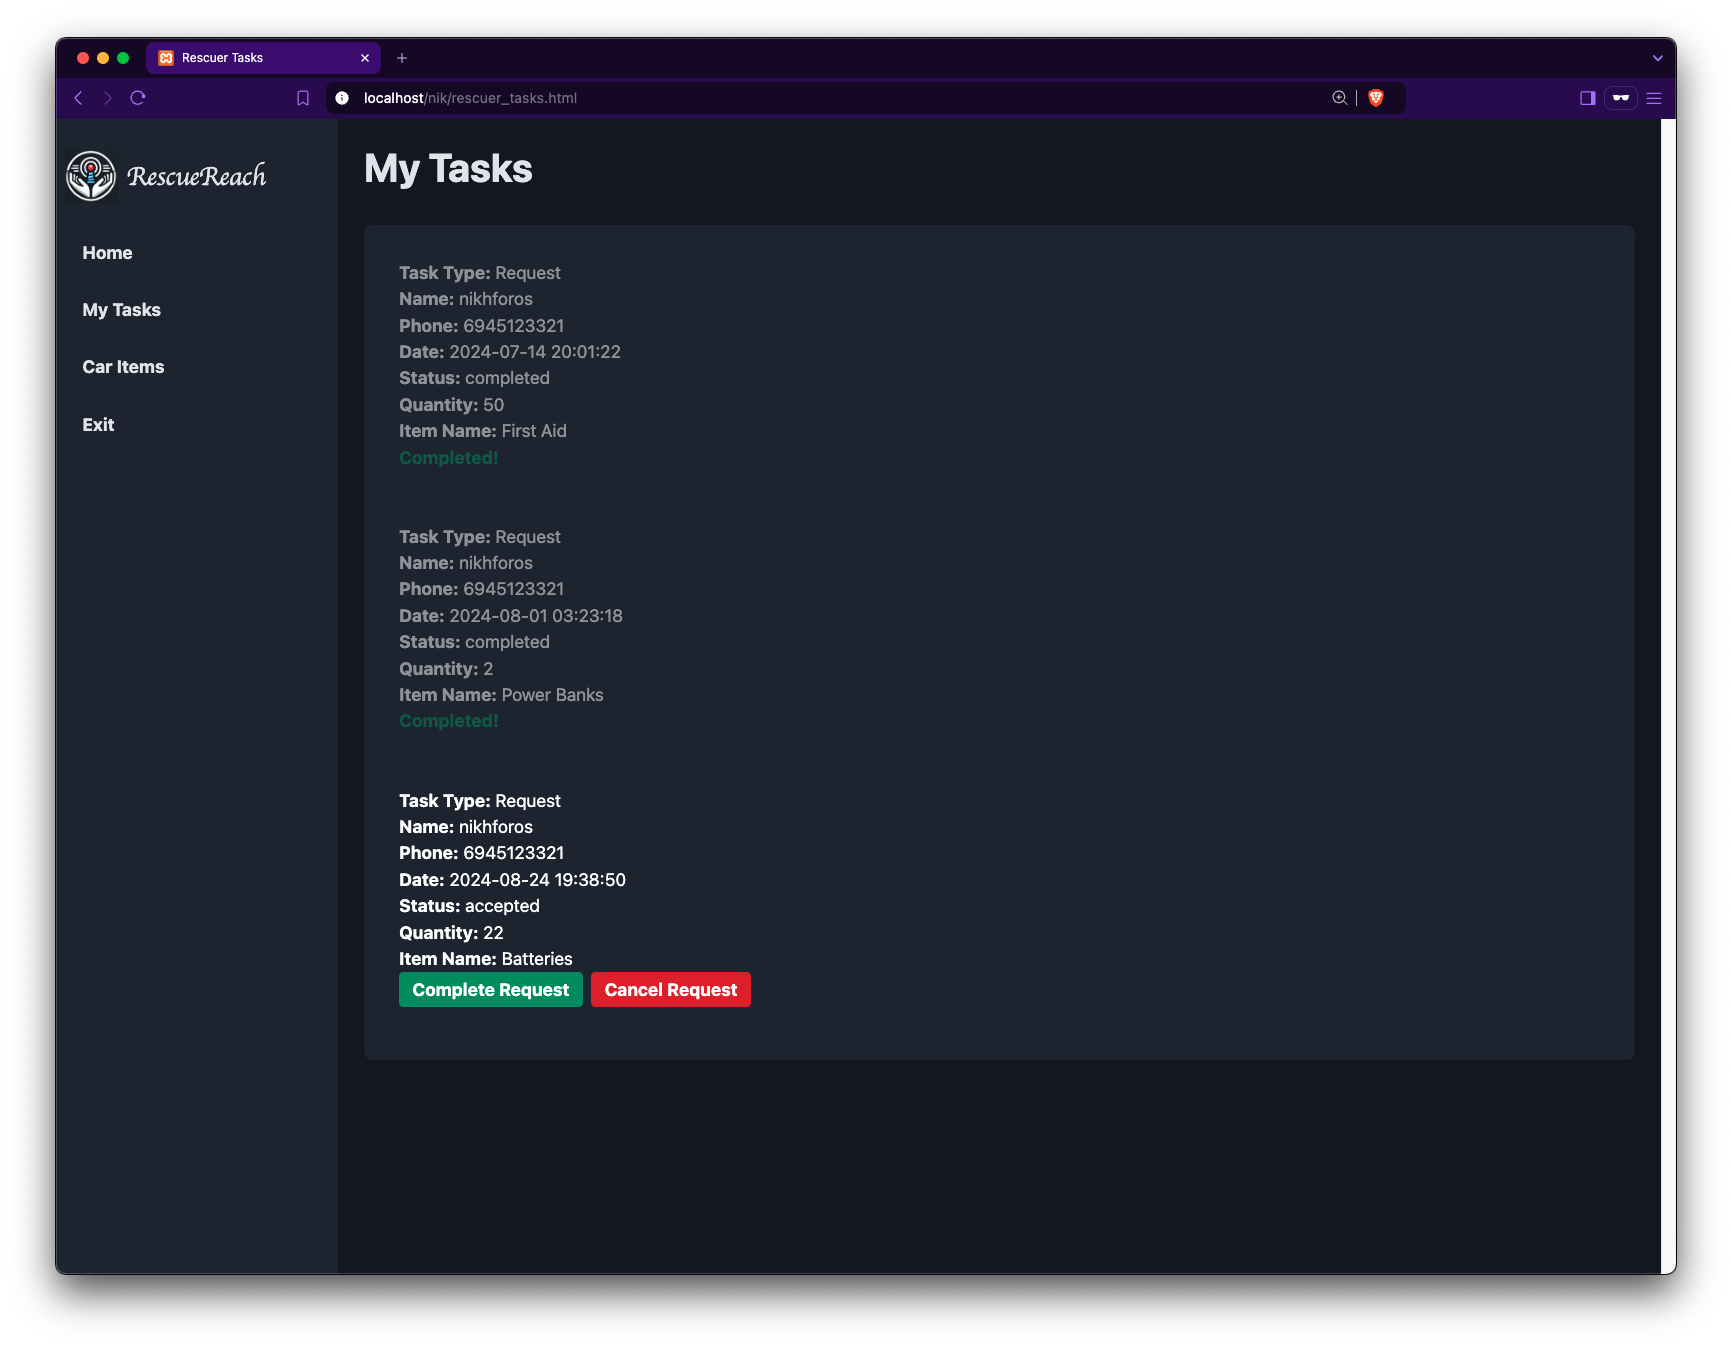
\includegraphics[width=0.7\textwidth]{img/rescuer-tasks}
            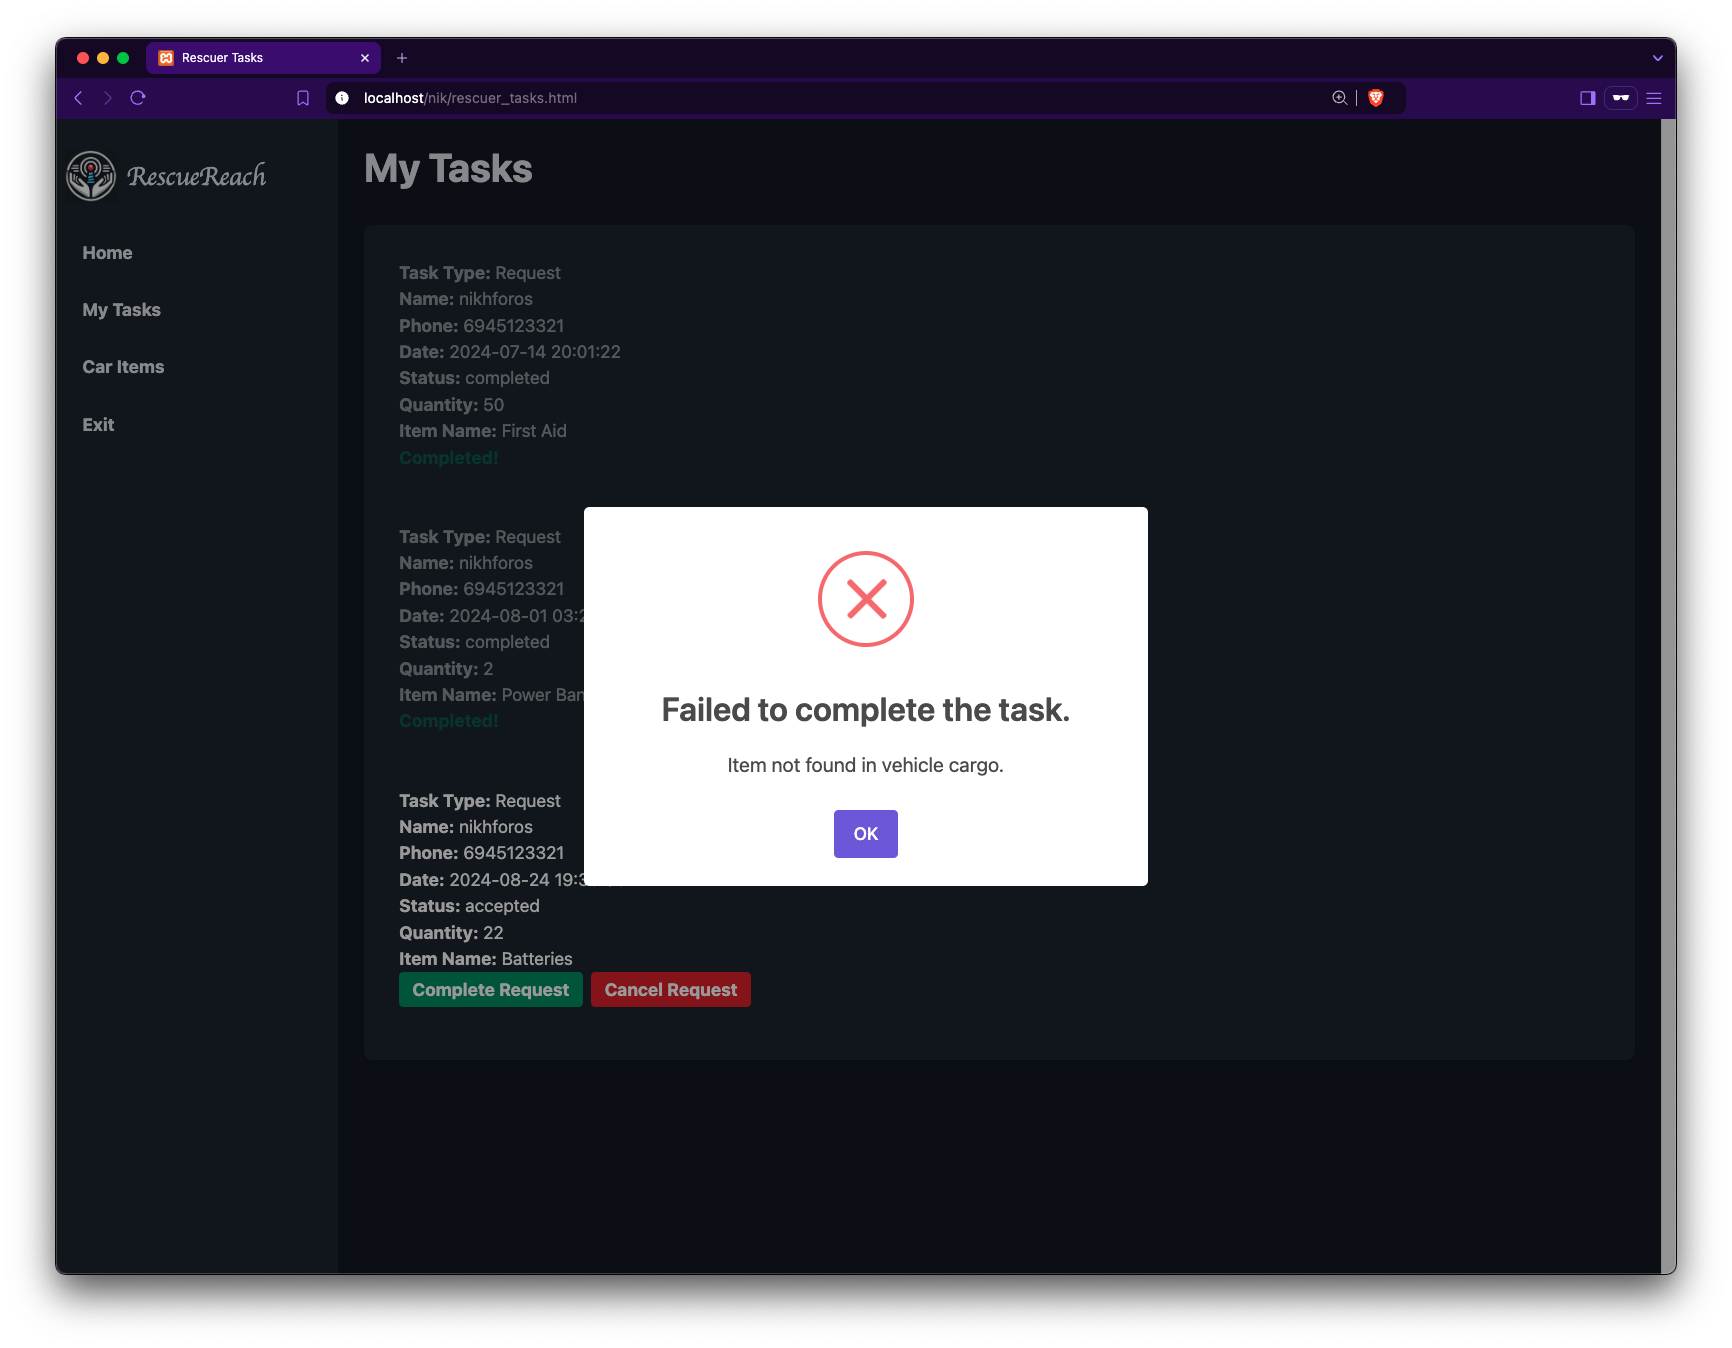
\includegraphics[width=0.7\textwidth]{img/rescuer-tasks-fail}
            \caption{Σελίδα με τα tasks του διασώστη}
        \end{figure}
        Κατά τη φόρτωση της σελίδας, γίνονται fetch τα tasks του διασώστη μέσω της \c{fetchRescuerTasks.php}, με συγκεκριμένο id ως \verb|rescuer_location.php?user_id=$={user_id}|,
            και αναπαραστάνονται μέσω της \c{displayTasks.php}.
        Αν ο διασώστης βρίσκεται κοντά σε κάποιον πολίτη, εμφανίζονται και οι επιλογές για \textbf{Complete Request/Offer} ή \textbf{Cancel Request/Offer}.
        Η λειτουργικότητα αυτών των επιλογών καθορίζεται από τις \c{completeTask()} και \c{cancelTask()} αντίστοιχα.

    \subsection{Items in Car}
        \begin{figure}[H] \noindent \centering
            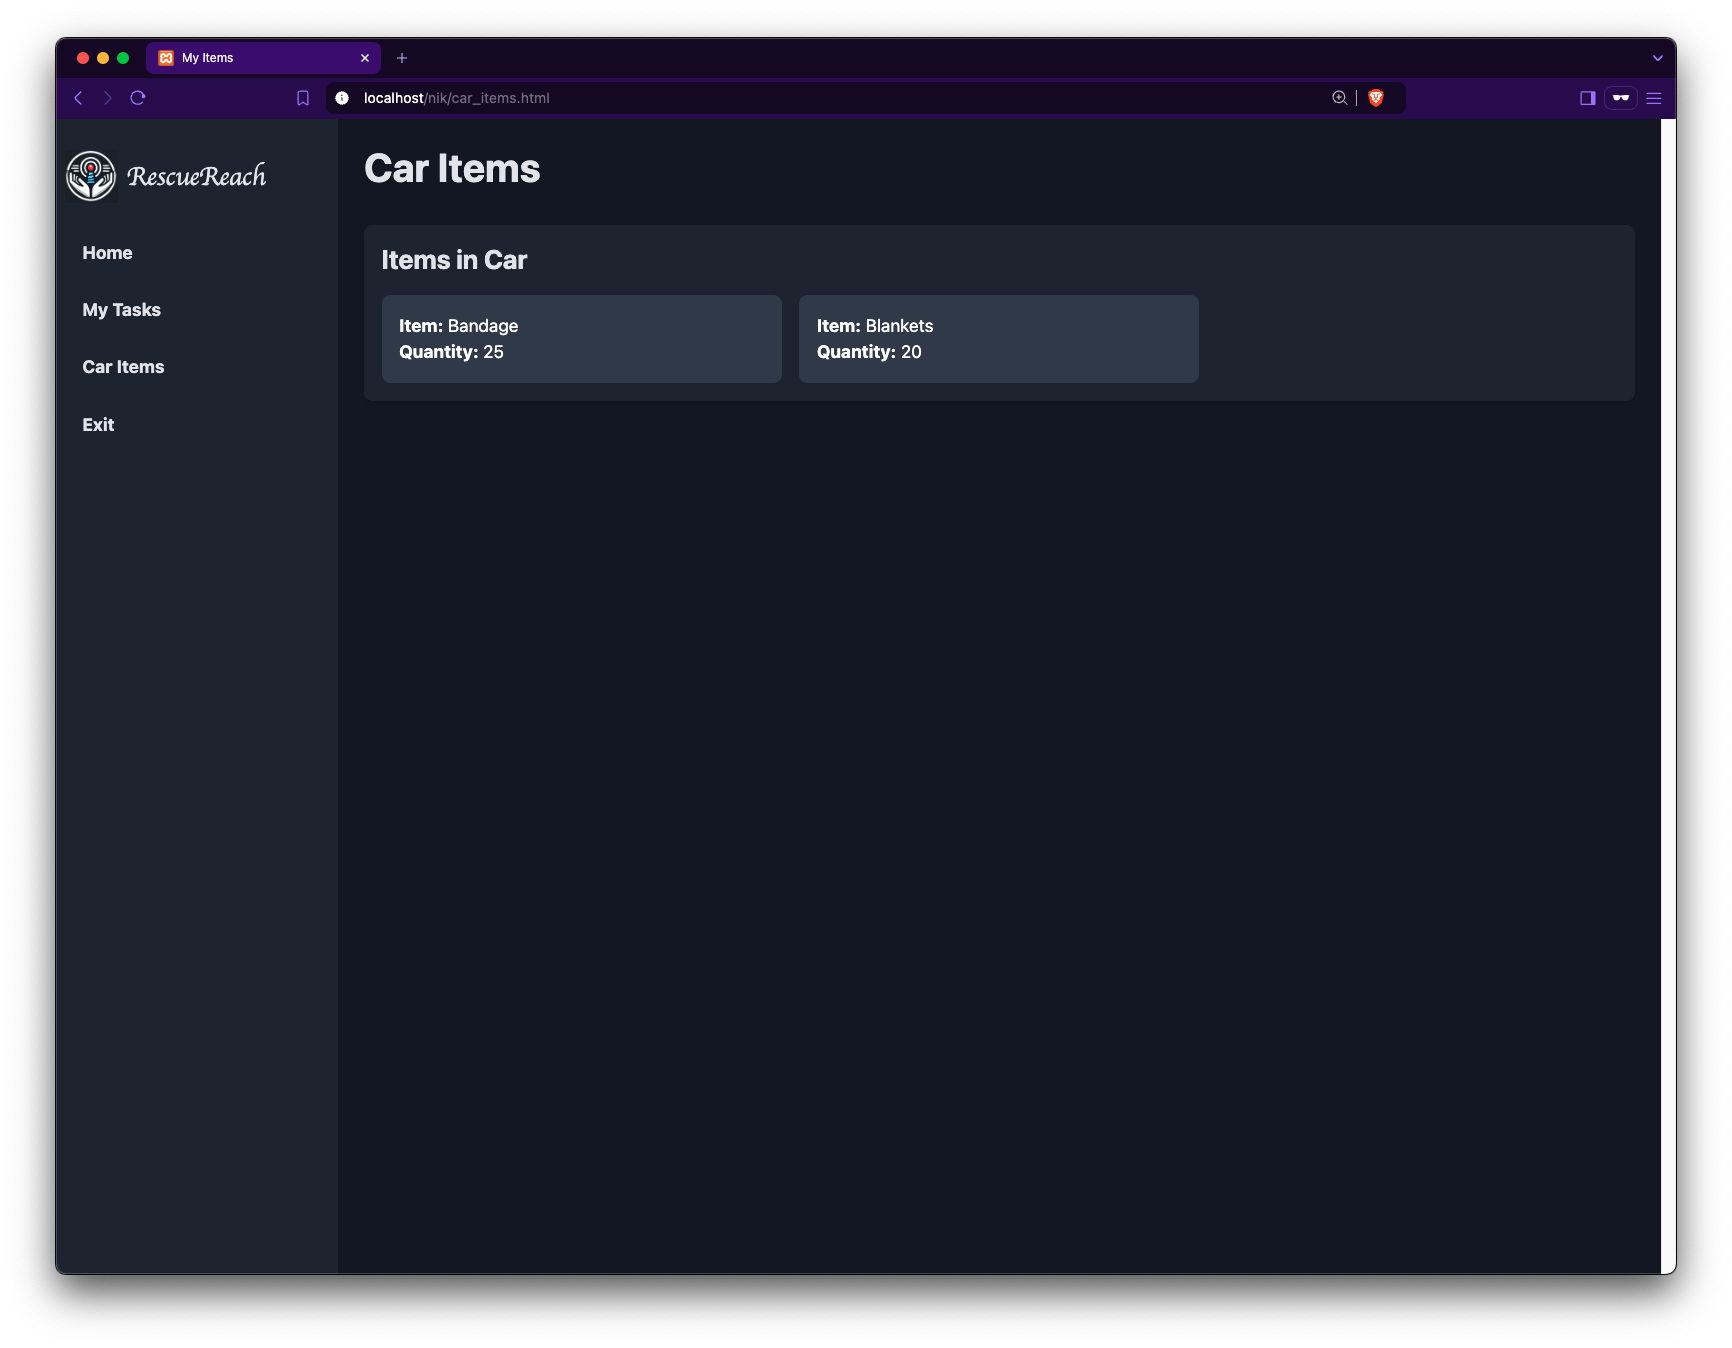
\includegraphics[width=0.8\textwidth]{img/rescuer-car_items}
            \caption{Inventory αντικειμένων διασώστη}
        \end{figure}

        Κατά τη φόρτωση της σελίδας, επιστρέφονται τα περιεχόμενα του αυτοκινήτου του διασώστη μέσω της \c{fetch\_items.php}.
        Η σελίδα δημιουργεί τις κάρτες με τα αντικείμενα μέσω της \c{display\_car\_items.php}.

    \subsection{Items in Base}
        \begin{figure}[H] \noindent \centering
            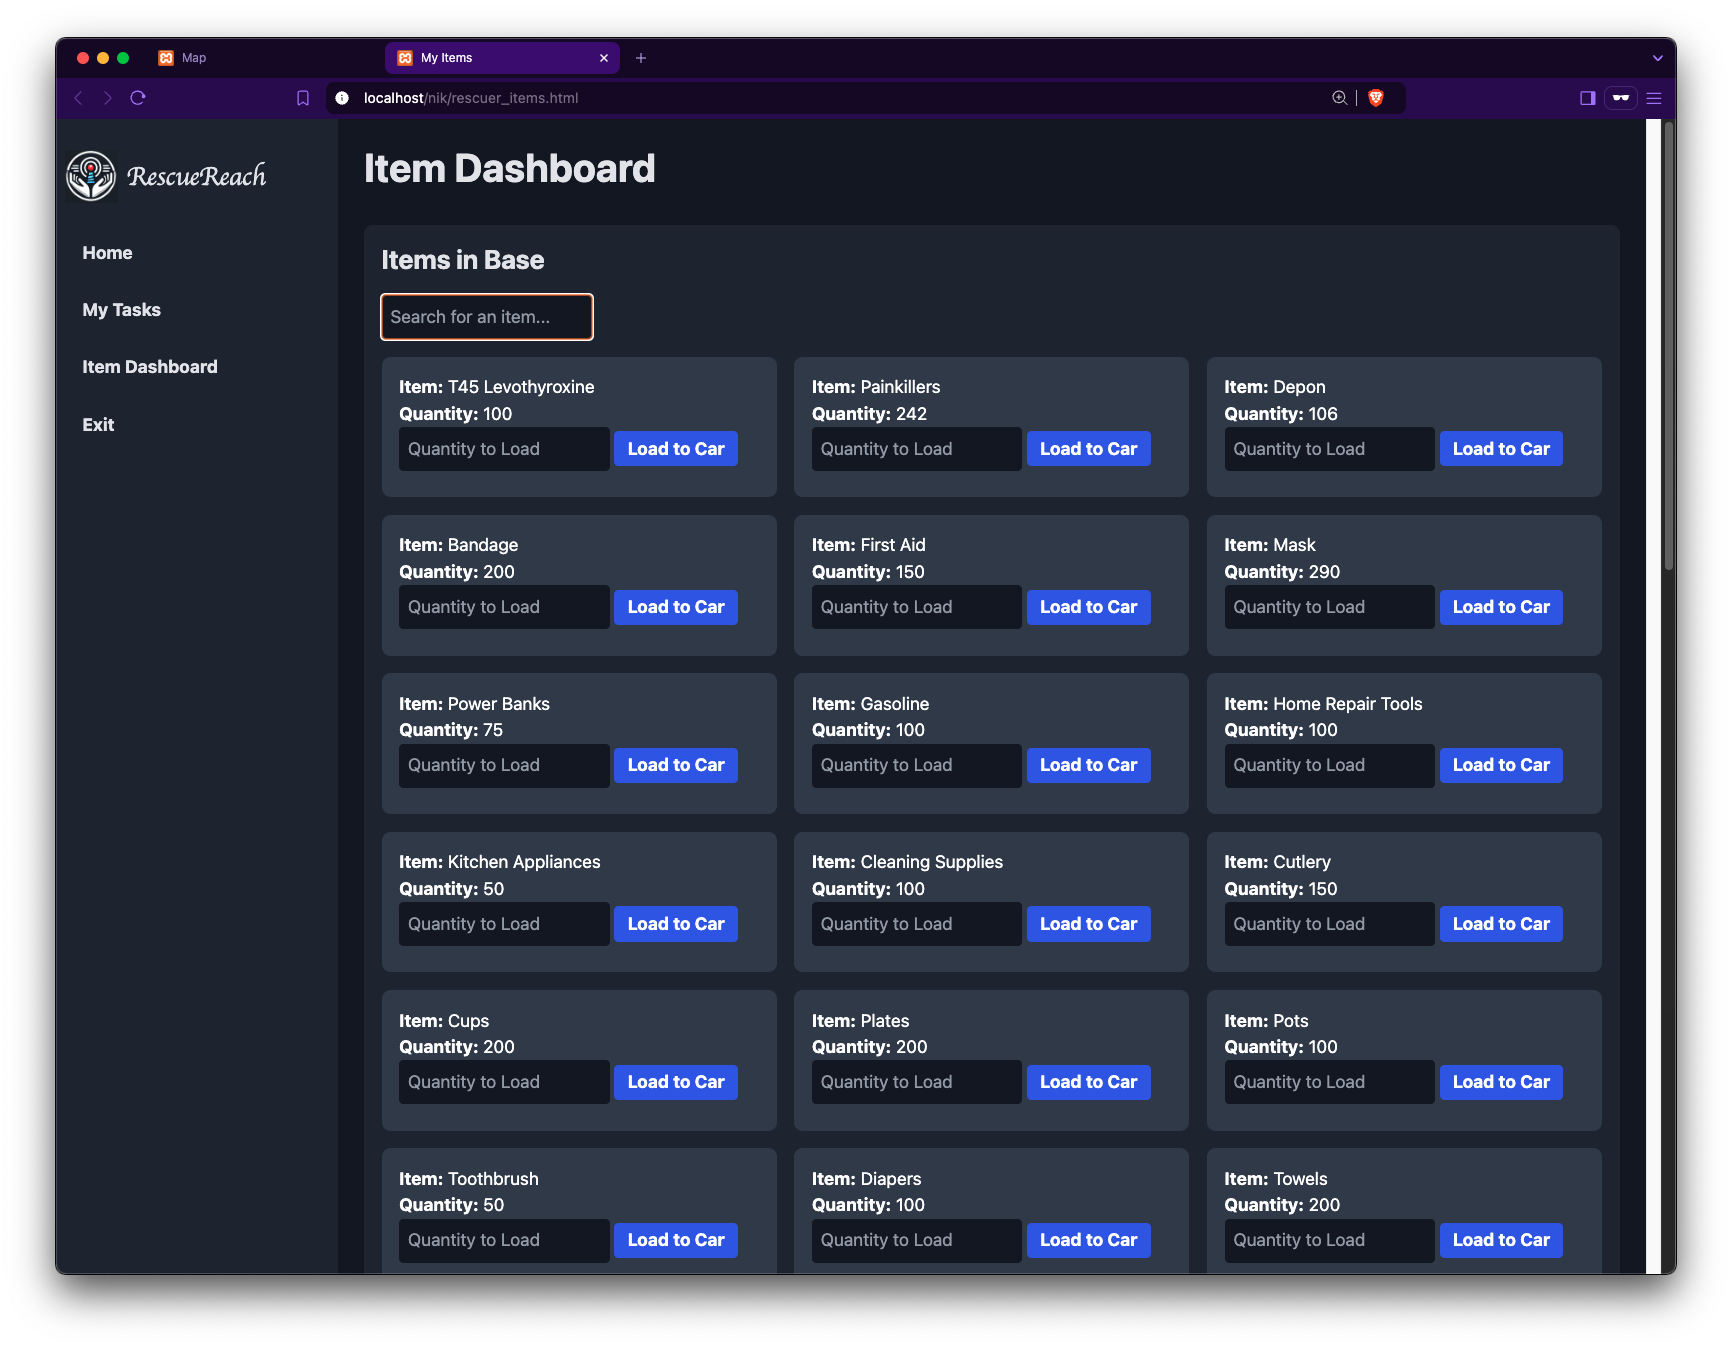
\includegraphics[width=0.8\textwidth]{img/rescuer-items_in_base}
            \caption{Μεταφορά αντικειμένων από/προς την βάση}
        \end{figure}

        Η σελίδα που εμφανίζεται όταν πατάμε στο \textbf{Load/Unload items}.
        Πάλι χρησιμοποιείται η \c{fetch\_items.php}, και τα περιεχόμενα εμφανίζονται μέσω της \c{displayBaseItems.php} και της \c{display\_car\_items.php}.
        Οι συναρτήσεις δημιουργούν επιπλέον και τα κατάλληλα κουμπιά με αντίστοιχους Event Listeners που καλούν τα \c{loadItemToCar()} (\c{load\_item.php}) και \c{unloadItemFromCar()} (\c{unload\_item.php}).